
% Preamble
\documentclass[12pt,a4paper]{article}

% Packages
\usepackage[utf8]{inputenc}
\usepackage[T1]{fontenc}
\usepackage{amsmath}
\usepackage{amsfonts}
\usepackage{amssymb}
\usepackage{graphicx}
\usepackage[margin=2.5cm]{geometry}
\usepackage{fancyhdr}

\usepackage{listings}          % For code snippets
\usepackage{xcolor}            % For colored text and boxes
\usepackage{tcolorbox}         % For nice looking boxes
\usepackage{enumitem}          % For better lists
\usepackage{tikz}              % For drawings and diagrams
\usepackage{mathtools}         % Enhanced math tools
\usepackage{tocloft}           % For customizing ToC
\usepackage{etoolbox}          % For patching commands
\usepackage{parskip}
\usepackage[spanish]{babel}
\usepackage{cite}
\usepackage{url}
\usepackage{hyperref}

\graphicspath{{images/}}
\bibliographystyle{unsrt}

\newcommand{\courseTitle}{Deep Learning}
\newcommand{\college}{Pontificia Universidad Católica del Perú}
\newcommand{\faculty}{Facultad de Ciencias e Ingeniería}
\newcommand{\courseCode}{1INF52}
\newcommand{\semester}{2025-0}
\newcommand{\noteDate}{\today}
\newcommand{\authors}{
    \begin{tabular}{@{}l@{\hspace{4em}}l@{}}
        Cántaro Márquez, Patricia Natividad & 20210907 \\[0.5cm]
        Nicho Manrique, Saymon Estefano & 20211866 \\[0.5cm]
        Zegarra Barrenechea, Carlos Eduardo & 20216177
    \end{tabular}
}

% for important notes
\newtcolorbox{important}[1]{
    colback=red!5!white,
    colframe=red!75!black,
    title=\textbf{#1}
}

% header and footer setup
\pagestyle{fancy}
\fancyhf{}
\rhead{\courseTitle}
\lhead{\courseCode}
\cfoot{\thepage}
\setlength{\headheight}{14.5pt}

\setlength{\parindent}{0pt}

% Document
\begin{document}

    \begin{titlepage}
    \centering
    % college
    \vspace*{0.5cm}
    {\Huge\bfseries \college \par}
    \vspace{1cm}
    {\Large\bfseries \faculty \par}
    \vspace{1cm}
    
\includegraphics[width=0.6\textwidth]{images/pucp}
    \vspace{2cm}

    % course
    {\Large\bfseries \courseTitle\ (\courseCode) \par}
    \vspace{1.5cm}
    {\large\bfseries Project Report \par}
    \vspace{2cm}
    \authors
    \vspace{2cm}

    % date
    {\large \noteDate \par}
    \vfill
\end{titlepage}
    \tableofcontents
    \newpage
    \section{Introducción}
Los incendios forestales representan una amenaza para el medio ambiente y la salud pública.
En la actualidad, su impacto ha aumentado por el cambio climático y el crecimiento
de la actividad humana en zonas boscosas (here). Estos eventos pueden partir de un origen
natural o antrópico (provocados, por ejemplo, por negligencia humana) y generan
consecuencias graves como daños en infraestructuras, pérdida de biodiversidad y
efectos económicos significativos.

La creciente frecuencia de incendios en bosques y otros biomas ha impulsado el desarrollo
de sistemas automáticos de vigilancia diseñados para detectar fuego y humo de manera
temprana, reduciendo el tiempo de respuesta de los equipos de extinción y minimizando
la propagación de los incendios.

El aprendizaje profundo (\textit{deep learning}) ha demostrado ser altamente eficaz
en el análisis de imágenes, especialmente para la detección de incendios y humo,
superando limitaciones presentes en métodos tradicionales. En este trabajo,
se desarrollará un modelo basado en estas tecnologías para...
    \section{Planteamiento del Problema}
A pesar de los avances en el uso de aprendizaje profundo para la detección de incendios,
muchas de las arquitecturas existentes no son lo suficientemente ligeras para ser
desplegadas en un dron, lo que limita su aplicabilidad en entornos de monitoreo aéreo
en tiempo real. Aunque existen modelos optimizados para dispositivos con restricciones
computacionales, muchos de ellos no han sido actualizados con las versiones más recientes
de arquitecturas de detección de objetos, lo que podría afectar su precisión y eficiencia.

Este trabajo busca abordar esta problemática explorando modelos que logren un equilibrio
entre precisión y eficiencia computacional, permitiendo su implementación efectiva en drones
para la detección temprana de incendios forestales.
    \section{Estado del Arte}


    \section{Marco Teórico}
El propósito de este marco teórico es introducir los conceptos clave que permitan abordar
la problemática de la detección de incendios forestales a partir del análisis de imágenes
con técnicas de \textit{deep learning}. Se explorarán las capacidades de las redes neuronales,
específicamente las redes neuronales convolucionales (CNNs), como herramientas a usar
para la detección y mitigación de estos eventos.

\subsection{Redes Neuronales Convolucionales}
Las redes neuronales convolucionales (CNNs) son un tipo de arquitectura de aprendizaje
profundo altamente efectiva para el procesamiento de datos que se pueden representar
como una cuadrícula, como lo son las imágenes. Su diseño les permite aprender de forma
automática jerarquías espaciales y patrones relevantes, lo cual las convierte en una
herramienta ideal para la claificación de imágenes y la detección de objetos.

Su arquitectura generalmente consta de tres tipos de capas principales: convolucionales,
de agrupación (\textit{pooling}) y completamente conectadas. Las capas convolucionales
aplican filtros a la imagen de entrada para extraer características relevantes, mientras
que las de agrupación reducen la dimensionalidad de las características extraídas.
Finalmente, las capas completamente conectadas se encargan de la clasificación final,
al asegurar que cada neurona de salida esté conectada a todas las neuronas de la capa
anterior.

El uso de CNNs en la detección de humo de incendios forestales se ha vuelto clave gracias
a su capacidad para procesar grandes volúmenes de datos visuales, como imágenes sateliteles
y transmisiones de cámaras de vigilancia. Esto permite diferenciar el humo de elementos
como nubes o niebla, y de forma más eficiente a diferencia de métodos tradicionales.

\subsection{Xception (Extreme Inception)}
Xception es una arquitectura basada en Inception que sustituye las convoluciones
estándar por \textit{depthwise separable convolutions}, lo que reduce la cantidad de
parámetros sin afectar el rendimiento. Separa la extracción de características en dos
etapas: primero filtra por canal y luego mezcla la información entre canales. Esto
permite un aprendizaje más eficiente y ha mostrado mejor rendimiento que InceptionV3
en conjuntos de datos grandes, aunque su implementación puede ser más costosa
computacionalmente en algunos casos \cite{sathishkumar_forest_2023}.


\subsection{DenseNet}
DenseNet optimiza el flujo de información conectando cada capa con todas las anteriores,
fomentando la reutilización de características y mejorando la propagación del gradiente.
Gracias a esta estructura, logra reducir el número de parámetros en comparación con otras
arquitecturas profundas sin perder precisión. Es útil para modelos muy profundos, pero su
alto número de conexiones puede aumentar el consumo de memoria durante el entrenamiento.

\subsection{ResNet}
ResNet introduce \textit{skip connections} o conexiones residuales que permiten que
los gradientes atraviesen varias capas sin degradarse, resolviendo el problema del
desvanecimiento del gradiente en redes profundas. En lugar de aprender transformaciones
completas, aprende diferencias entre la entrada y la salida esperada, lo que facilita
el entrenamiento y permite construir redes con cientos de capas. Aunque es altamente
eficiente, las versiones más profundas pueden requerir un ajuste cuidadoso de
hiperparámetros para evitar sobrecostos computacionales \cite{sathishkumar_forest_2023}.

\subsection{YOLO}
You Only Look Once es un modelo avanzaado de detección de objetos diseñado para identificar
y localizar elemntos en imágenes en tiempo real con alta precisión. Su funcionamiento se
basa en redes neuronales convolucionales (CNNs) para analizar imágenes con un solo
procesamiento, dividiéndolas en cuadrículas y prediciendo la posición, dimensiones y
clase de los objetos detectados \cite{yaseen2024yolov8indepthexplorationinternal}.

YOLOv8, la versión más reciente, introduce un enfoque sin anclas (\textit{anchor-free}),
eliminando las posiciones predefinidas de las cajas delimitadoras usadas en versiones
anteriores. Esto le ayuda a simplificar el entrenamiento y mejorar la precisión en la
detección de objetos con formas y tamaños variables. Además, incorpora CSPNet
(\textit{Cross-Stage Partial Networks}) como backbone, una arquitectura que optimiza el
flujo de información y reutiliza características de capas anteriores para reducir las
redundancias y mejorar la eficiencia computacional.

Estas características le permiten a YOLOv8 servir como herramienta altamente eficaz para
tareas en tiempo real, y para actividades de vigilancia y monitoreo ambiental como es el
caso de la detección de incendios forestales \cite{s23208374}.

\subsection{Transfer Learning}
El aprendizaje por transferencia es una técnica de aprendizaje automático que consiste
en reutilizar conocimientos aprendidos en un dominio para mejorar el rendimiento en otro
dominio relacionado. En el contexto de las redes neuronales, esto implica tomar una red
preentrenada en un conjunto de datos grande y ajustarla a un conjunto de datos más
pequeño y específico.

    \section{Propuesta de Modelo}

\subsection{Dataset}
Se usará el FLAME dataset \cite{FLAME_Dataset} ya que este ha sido diseñado para estudios de
detección y segmentación de incendios, conteniendo imágenes y videos capturados mediante
drones en bosques del norte de Arizona. Para este proyecto, se usarán solo las imágenes y
se aprovechará que estas ya han sido distribuidas y etiquetadas para ser usadas:
39,375 imágenes para entrenamiento/validación y 8,617 imágenes para testeo.

\subsection{Arquitectura Propuesta}
Con el dataset de FLAME, se usará un ensamble de 3 modelos, los cuales serán: Xception,
DenseNet y ResNet; y posteriormente se destilarán en un modelo ligero como lo es
MobileNetV3. Además, se usarán ténicas de pruning antes del deployment para reducir
el tamaño del modelo y mejorar la eficiencia en la inferencia.

\begin{figure}[h]
    \centering
    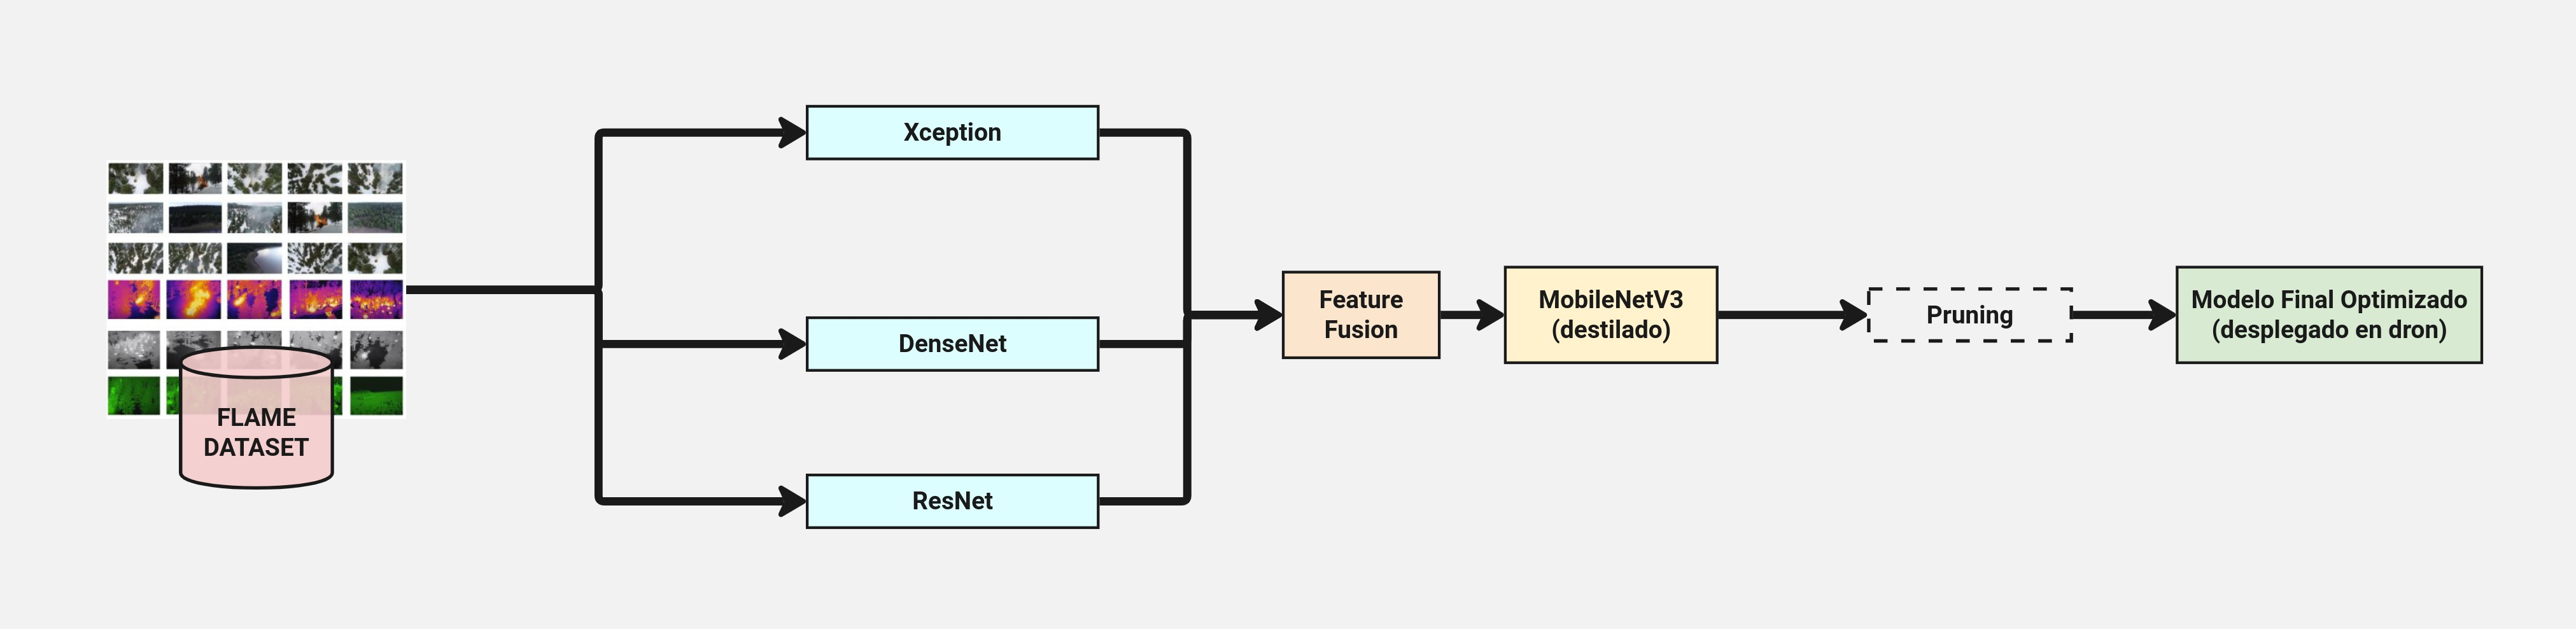
\includegraphics[width=0.9\textwidth]{images/model}
    \caption{Descripción del modelo}
    \label{fig:model}
\end{figure}

Se utilizarán \textbf{CNNs entrenadas sobre el dataset FLAME}, específicamente:

\begin{itemize}
    \item \textbf{Xception}: Utiliza \textit{Depthwise Separable Convolutions (DSC)} para optimizar la extracción de características, capturando relaciones complejas en la imagen. Se considera más eficiente en comparación con arquitecturas tradicionales.
    \item \textbf{DenseNet}: Usa \textit{bloques densos} que facilitan la reutilización de características, beneficiando la detección de elementos sutiles como \textit{ríos o humo de bajo contraste}.
    \item \textbf{ResNet}: Implementa \textit{conexiones residuales} para evitar la degradación del gradiente en redes profundas, lo que mejora la convergencia en entrenamientos largos.
\end{itemize}

\subsubsection{Entrenamiento previo al ensamble}
Cada modelo se entrenará \textbf{de manera individual} para la clasificación de incendios, empleando \textit{cross-entropy} como función de pérdida y aplicando \textit{early stopping} para evitar el sobreajuste.

\subsubsection{Fusión de Modelos (Ensamble)}
Una vez completados los entrenamientos individuales, se procederá con la fusión de modelos. Se consideran dos estrategias:

\begin{enumerate}
    \item \textbf{Fusión a nivel de salidas finales}:
    \begin{itemize}
        \item Se combinan las \textit{probabilidades} generadas por los tres modelos en un vector mayor.
        \item Se ajusta el \textit{peso} de cada modelo y se valida con \textit{cross-validation}.
    \end{itemize}

    \item \textbf{Fusión en capas intermedias}:
    \begin{itemize}
        \item Se extraen \textit{vectores de características} desde capas intermedias de cada modelo y se concatenan en un vector mayor.
        \item Se entrena un \textit{clasificador adicional} sobre este vector fusionado para generar la salida final.
    \end{itemize}
\end{enumerate}

\subsubsection{Knowledge Distillation}
Dado que el ensamble es \textbf{demasiado grande} para dispositivos con recursos limitados, se aplicará \textit{Knowledge Distillation}. Se entrenará un \textbf{MobileNetV3} como versión comprimida del ensamble, preservando la mayor cantidad de información relevante.

\subsubsection{Optimización Adicional: Pruning}
Para reducir aún más el tamaño del modelo, se aplicará \textit{pruning}, eliminando \textbf{pesos irrelevantes o de magnitud baja}. Esto permite reducir la carga computacional sin afectar significativamente la precisión.

\subsection{Justificación}

\begin{itemize}
    \item \textbf{Uso de Xception, DenseNet y ResNet en paralelo:}
    \begin{itemize}
        \item \textbf{Xception}: Usa convoluciones separables, reduciendo cálculos sin perder precisión.
        \item \textbf{DenseNet}: Mejora reutilización de características, ideal para detectar detalles pequeños.
        \item \textbf{ResNet}: Usa conexiones residuales, facilitando el entrenamiento en redes profundas.
    \end{itemize}
    \item \textbf{Destilación en MobileNetV3:}
    \begin{itemize}
        \item Modelo ligero y eficiente para \textit{drones}.
        \item Mantiene precisión al aprender de los modelos grandes.
    \end{itemize}
    \item \textbf{Ventajas sobre el estado del arte:}
    \begin{itemize}
        \item Más eficiente que ViT y ResNet en inferencia en dispositivos de bajo consumo.
        \item Mejor precisión que modelos CNN individuales.
    \end{itemize}
    \item \textbf{Despliegue en \textit{drones}:}
    \begin{itemize}
        \item Menor consumo de energía que ViT y CNNs pesados.
        \item Inferencia en tiempo real en \textit{Jetson Nano, Coral TPU, Raspberry Pi}.
    \end{itemize}
\end{itemize}


    
    % \include{contents/experimentation}
    % \section{Conclusions and Future Work}
\label{sec:conclusions}

\begin{itemize}
    \item \textbf{DenseNet121} achieved the best accuracy (86.50\%) on FLAME, with an
    F1-score of 0.8324.
    \item The \textbf{ensemble} of Xception, DenseNet, and ResNet delivers consistent
    performance (79.40\% accuracy), though it does not surpass DenseNet alone.
    \item \textbf{Keras Tuner} guided hyperparameter tuning, significantly improving
    each individual model's performance.
    \item \textbf{Future Directions:}
      \begin{enumerate}
        \item \textbf{Knowledge Distillation:} Compress the ensemble into MobileNetV3
        for lighter deployments on drones.
        \item \textbf{Pruning:} Reduce unnecessary weights to speed up inference.
        \item \textbf{Vision Transformers (ViTs):} Integrate and compare them against
        the CNN ensemble.
      \end{enumerate}
\end{itemize}

In summary, this project underscores the potential of deep learning for near-real-time
wildfire detection and opens the path for efficient aerial monitoring systems.

\textbf{Acknowledgment:} Credit must be given to all three members of \textbf{CPSquad},
as they contributed equally to this work.


    \newpage
    \bibliography{../contents/references}

\end{document}